% Created 2020-08-29 Sat 00:45
% Intended LaTeX compiler: pdflatex
\documentclass[presentation]{beamer}
\usepackage[utf8]{inputenc}
\usepackage[T1]{fontenc}
\usepackage{graphicx}
\usepackage{grffile}
\usepackage{longtable}
\usepackage{wrapfig}
\usepackage{rotating}
\usepackage[normalem]{ulem}
\usepackage{amsmath}
\usepackage{textcomp}
\usepackage{amssymb}
\usepackage{capt-of}
\usepackage{hyperref}
\usepackage{etex}
\usepackage{amsmath}
\usepackage{pstricks}
\usepackage{pgfplots}
\usepackage{tikz}
\usepackage[europeanresistors,americaninductors]{circuitikz}
\usepackage{colortbl}
\usepackage{yfonts}
\usetikzlibrary{shapes,arrows}
\usetikzlibrary{positioning}
\usetikzlibrary{arrows,shapes}
\usetikzlibrary{intersections}
\usetikzlibrary{calc,patterns,decorations.pathmorphing,decorations.markings}
\usepackage[BoldFont,SlantFont,CJKchecksingle]{xeCJK}
\setCJKmainfont[BoldFont=SimHei]{KaiTi}
\setCJKmonofont{KaiTi}
\usepackage{pst-node}
\usepackage{pst-plot}
\psset{unit=5mm}
\mode<beamer>{\usetheme{Frankfurt}}
\mode<beamer>{\usecolortheme{dove}}
\mode<article>{\hypersetup{colorlinks=true,pdfborder={0 0 0}}}
\AtBeginSection[]{\begin{frame}<beamer>\frametitle{Topic}\tableofcontents[currentsection]\end{frame}}
\setbeamercovered{transparent}
\usetheme{default}
\date{}
\title{绪论}
\hypersetup{
 pdfauthor={},
 pdftitle={绪论},
 pdfkeywords={},
 pdfsubject={},
 pdfcreator={Emacs 25.3.1 (Org mode 9.3.6)}, 
 pdflang={English}}
\begin{document}

\maketitle
\begin{frame}{Outline}
\tableofcontents
\end{frame}









\section{计算视觉与模式识别历史与发展;}
\label{sec:org75751dc}

\begin{frame}[label={sec:orgaf7cadf}]{什么是计算机视觉?}
\begin{itemize}
\item 计算机视觉本质上就是研究视觉感知问题。
\item 视觉感知是指对“环境表达和理解中,对视觉信息的组织、识别和解释的过程
\item 计算机视觉的目标是对环境的表达和理解
\item 核心问题是研究如何对输入的图像信息进行组织,对物体和场景进行识别,进而对图像内容给予解释。
\end{itemize}
\end{frame}

\begin{frame}[label={sec:org07d505f}]{计算机视觉历史}
\begin{itemize}
\item 1982年马尔( David Marr )《视觉》(Marr, 1982)一书问世
\item 马尔的计算视觉分为三个层次: 计算理论、表达和算法以及算法实现。
\end{itemize}
\end{frame}

\begin{frame}[label={sec:orgf427d24}]{David Marr}
\begin{center}
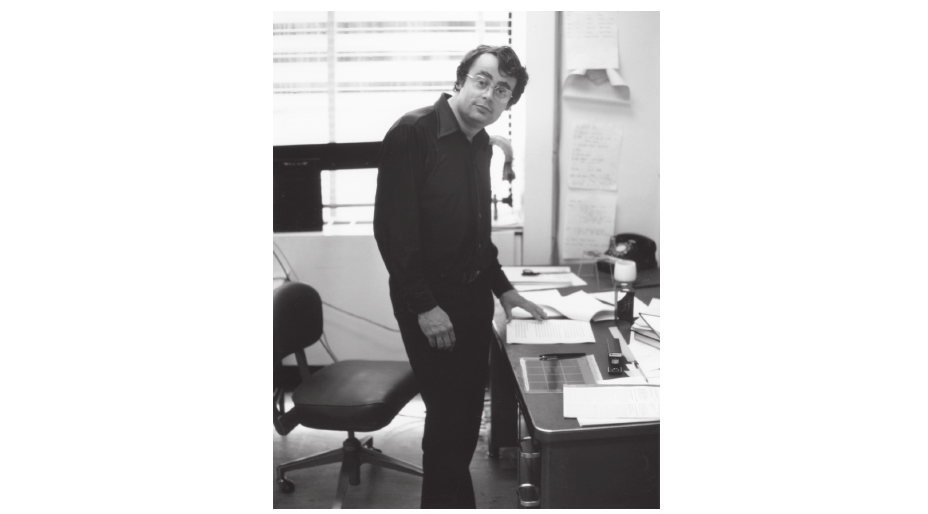
\includegraphics[width=.9\linewidth]{./image/David Marr at MIT.png}
\end{center}
\end{frame}

\begin{frame}[label={sec:org391e914}]{计算理论(Computational Theory)}
\begin{itemize}
\item 视觉不管有多少功能,主要功能在于“从视网膜成像的二维图像来恢复空间物体的可见三维表面形状”,称之为“三维重建”(3D reconstruction)。而且,这种重建过程可以通过计算完成。
\item 图像是物理空间在视网膜上的投影,所以图像信息蕴含了物理空间的内在信息,因此,任何计算视觉计算理论和方法都应该从图像出发,充分挖掘图像所蕴含的对应物理空间的内在属性。
\end{itemize}
\end{frame}

\begin{frame}[label={sec:orge4055c3}]{表达和算法(Representationand Algorithm)}
\begin{itemize}
\item 马尔视觉计算理论的“物体表达”,是指“物体坐标系下的三维形状表达”。同一物体,选用的坐标系不同,表达方式亦不同。
\item 马尔将“观测者坐标系下的三维几何形状表达”称之为“2.5维表达”,物体坐标系下的表达为“三维表达”。
\end{itemize}
\end{frame}

\begin{frame}[label={sec:org6d8aab1}]{批评}
\begin{itemize}
\item 认为这种三维重建过程是“纯粹自底向上的过程”(pure bottom-up process),缺乏高层反馈(top-down feedback);
\item “重建”缺乏“目的性和主动性”。由于不同的用途,要求重建的精度不同,而不考虑具体任务,仅仅“盲目地重建一个适合任何任务的三维模型”似乎不合理。
\end{itemize}
\end{frame}

\begin{frame}[label={sec:orgcf87d52}]{多视几何(Multiple View Geometry)}
\begin{itemize}
\item “多视几何”本质上就是研究射影变换下图像对应点之间以及空间点与其投影的图像点之间的约束理论和计算方法的学科。
\item 计算机视觉领域,多视几何主要研究二幅图像对应点之间的对极几何约束(epipolar geometry), 三幅图像对应点之间的三焦张量约束(tri-focal tensor),空间平面点到图像点,或空间点为平面点投影的多幅图像点之间的单应约束(homography)等。
\end{itemize}
\end{frame}

\begin{frame}[label={sec:org8738c66}]{分层三维重建(Stratified 3D Reconstruction)}
\begin{itemize}
\item 从多幅二维图像恢复欧几里德空间的三维结构时,不是从图像一步到欧几里德空间下的三维结构,而是分步分层地进行。
\item 先从多幅图像的对应点重建射影空间下的对应空间点(即射影重建:projective reconstruction),
\item 然后把射影空间下重建的点提升到仿射空间下(即仿射重建:affine reconstruction),
\item 最后把仿射空间下重建的点再提升到欧几里德空间(或度量空间: metric reconstruction)
\end{itemize}
\end{frame}

\begin{frame}[label={sec:orga074b08}]{什么是模式识别?}
模式识别研究的目的是利用计算机对物理对象进行分类,在错误概率最小的条件下,使识别的结果尽量与客观物体相符合。
\end{frame}

\begin{frame}[label={sec:org0d7648f}]{模式识别历史}
\begin{itemize}
\item 二十世纪三十年代,Fisher提出统计分类理论,奠定了统计模式识别的基础。
\item 二十世纪六十年代,L.A.Zadeh 提出模糊集理论,模糊模式识别方法得以发展和应用。
\item 二十世纪八十年代,以Hopfield网络、BP网络为代表的神经网络模型导致了人工神经网络的复活,并且在模式识别领域得到了比较广泛的应用。
\item 二十世纪九十年代,小样本学习理论、支持向量机方法被提出(由 Corinna Cortes 和 Vapnik 提出)。
\item 2000年,流形学习被提出(manifold learning)。
\item 2005年,稀疏表示(sparse representation)的方法被提出。
\item 2006年,深度学习的概念被 Hinton 等人提出。Yan Lecun 等人又提出卷积神经网络。
\end{itemize}
\end{frame}

\section{计算视觉与模式识别应用介绍;}
\label{sec:org8a33332}

\begin{frame}[label={sec:org7cbe811}]{计算机视觉示例}
\begin{itemize}
\item 无人驾驶汽车
\item 手写识别
\item 人脸识别
\end{itemize}
\end{frame}


\begin{frame}[label={sec:orgc463a14}]{ALVINN [Pomerleau] drives 70 mph on highways}
\begin{center}
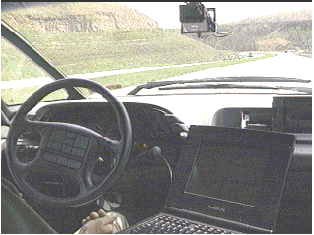
\includegraphics[width=.9\linewidth]{./image/nl5-interior-front-color.png}
\end{center}
\begin{center}
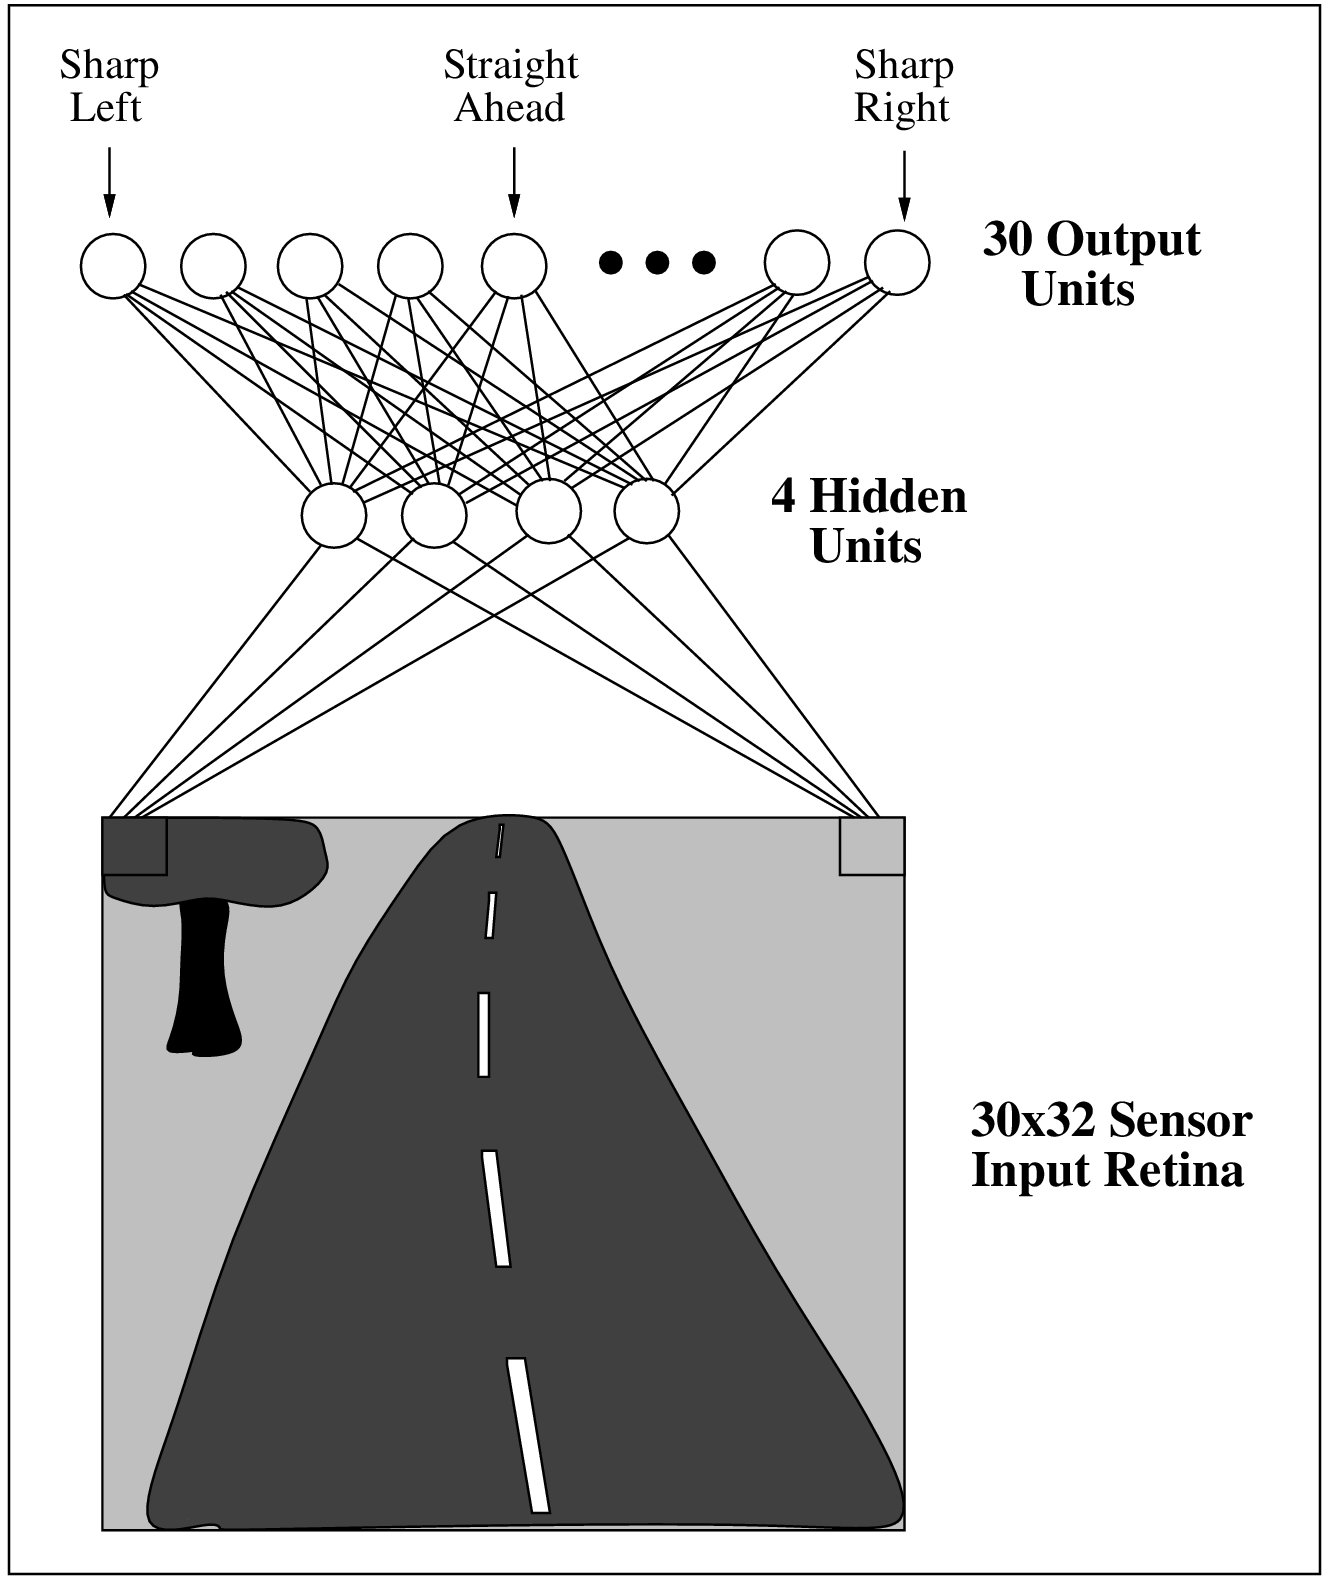
\includegraphics[width=.9\linewidth]{./image/alvinn1.png}
\end{center}
\begin{center}
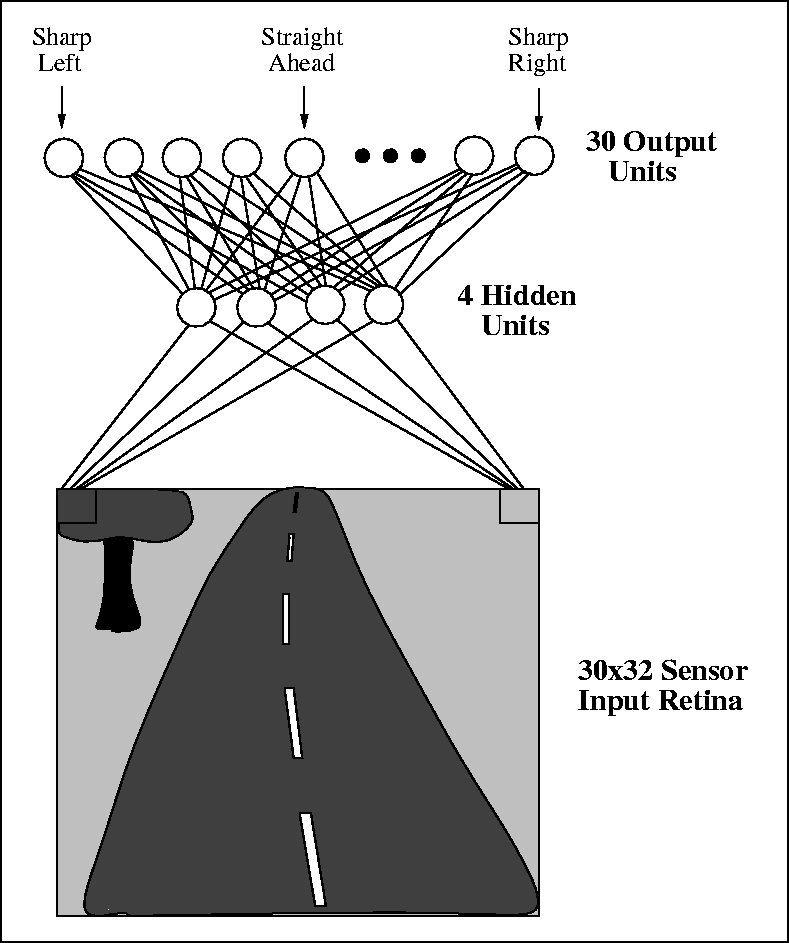
\includegraphics[width=.9\linewidth]{./image/alvinn2.png}
\end{center}
\end{frame}


\begin{frame}[label={sec:org83fefa4}]{示例:三维场景重建}
\begin{center}
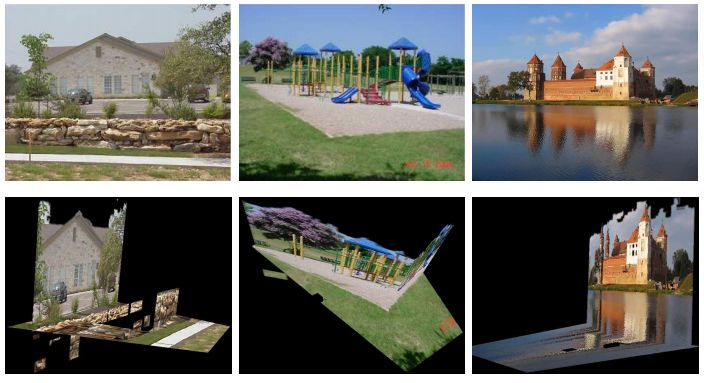
\includegraphics[width=.9\linewidth]{./image/scene.jpg}
\end{center}
\end{frame}




\section{课程简介}
\label{sec:org3024e2d}

\begin{frame}[label={sec:org42799cb}]{课程主要内容}
\begin{itemize}
\item 摄像机标定
\item 图像特征提取
\item 图像配准与拼接
\item 立体视觉
\item 模式识别基础
\item 图像目标识别
\item 运动分析
\end{itemize}
\end{frame}

\begin{frame}[label={sec:orgdefc866}]{与其它课程关系}
\begin{itemize}
\item 概率与数理统计
\item 图像处理
\item 人工智能
\item 机器学习
\item 模式识别
\item 心理学
\item 哲学
\end{itemize}
\end{frame}


\section{相关资源}
\label{sec:org7429d4a}
\begin{frame}[label={sec:org46c112f}]{文献资源}
\begin{itemize}
\item TPAMI: IEEE Trans on Pattern Analysis and Machine Intelligence
\item IJCV: International Journal of Computer Vision
\item TIP: IEEE Transactions on Image Processing
\item TNNLS: IEEE Transactions on Neural Networks and learning systems
\item Pattern Recognition
\end{itemize}
\end{frame}
\begin{frame}[label={sec:orgfcd297a}]{会议}
\begin{itemize}
\item ICCV: International Conference on Computer Vision
\item CVPR: International Conference on Computer Vision and Pattern Recognition
\item ECCV: European Conference on Computer Vision
\item ICML: International Conference on Machine Learning
\item NIPS: Annual Conference on Neural Information Processing Systems
\item AAAI: AAAI Conference on Artificial Intelligence
\end{itemize}
\end{frame}

\begin{frame}[label={sec:org91832f2}]{课程}
\begin{itemize}
\item \url{https://www.coursera.org/learn/machine-learning}  Machine Learning Stanford University (coursera)
\item \url{http://open.163.com/special/opencourse/machinelearning.html}  斯坦福大学公开课 :机器学习课程(网易公开课)
\item \url{http://open.163.com/special/opencourse/learningfromdata.html} 加州理工学院公开课:机器学习与数据挖掘
\end{itemize}
\end{frame}

\begin{frame}[label={sec:org6c49f4c}]{资料}
\begin{itemize}
\item \url{https://www.kaggle.com/}
数据科学竞赛平台、社区
\item \url{http://philschatz.com/biology-book/}  
a  freedom book about biology
\item \href{http://www.cs.cmu.edu/\~tom/mlbook-chapter-slides.html}{http://www.cs.cmu.edu/\textasciitilde tom/mlbook-chapter-slides.html}
Machine Learning slide (\LaTeX{} source )
\item \url{http://www.cs.cmu.edu/afs/cs.cmu.edu/project/theo-20/www/mlbook/latex-support.html} 
Machine Learning slide (\LaTeX{} source )
\item \url{https://learnxinyminutes.com}
各种程序设计语言快速入门
\item \url{http://cos.name/}
统计技术社区
\item \url{https://databricks.com/}
Spark在线学习
\end{itemize}
\end{frame}

\section{工具}
\label{sec:org81a800d}
\begin{frame}[label={sec:org40503fa}]{C/C++}
\begin{itemize}
\item \url{http://dlib.net}
\item \url{http://mlpack.org/}
\item \url{http://opencv.org/}
\item \url{http://caffe.berkeleyvision.org}
\item \url{http://mxnet.io/}
\end{itemize}
\end{frame}

\begin{frame}[label={sec:org3bd7f83}]{Lua}
\begin{itemize}
\item \url{http://torch.ch}
\item \url{https://github.com/torchnet/}
\end{itemize}
\end{frame}

\begin{frame}[label={sec:org448ce83}]{Python}
\begin{itemize}
\item \url{http://scikit-image.org/}
\item \url{http://scikit-learn.org/}
\item \url{http://programmingcomputervision.com/}
\item \url{https://www.tensorflow.org}
\item \url{https://pytorch.org/}
\end{itemize}
\end{frame}

\begin{frame}[label={sec:org3ed9c69}]{Java}
\begin{itemize}
\item \url{http://www.cs.waikato.ac.nz/ml/weka/index.html}
\item \url{http://moa.cms.waikato.ac.nz/}
\item \url{http://spark.apache.org/mllib/}
\item \url{https://mahout.apache.org/}
\item \url{http://www.h2o.ai/}
\item \url{http://deeplearning4j.org/}
\item \url{http://neuroph.sourceforge.net/}
\item \url{http://airbnb.io/aerosolve/}
\end{itemize}
\end{frame}

\begin{frame}[label={sec:org8b2adc1}]{科学计算}
\begin{itemize}
\item Rstudio(R)
\item Matlab/Octave
\item Scilab
\item Sage
\item Julia
\item Spyder(Python)
\item RapidMiner \url{https://rapidminer.com/}
\end{itemize}
\end{frame}
\end{document}